%%%%%%%% ICML 2018 EXAMPLE LATEX SUBMISSION FILE %%%%%%%%%%%%%%%%%

\documentclass{article}

% Recommended, but optional, packages for figures and better typesetting:
\usepackage{microtype}
\usepackage{graphicx}
\graphicspath{{./figs/}}
\usepackage{subfigure}
\usepackage{booktabs} % for professional tables

\usepackage{amsmath,amssymb,amsfonts,amsthm,amscd,bm,bbm}
\usepackage{mathtools}

% hyperref makes hyperlinks in the resulting PDF.
% If your build breaks (sometimes temporarily if a hyperlink spans a page)
% please comment out the following usepackage line and replace
% \usepackage{icml2018} with \usepackage[nohyperref]{icml2018} above.
\usepackage{hyperref}
\usepackage[inline]{enumitem}
\usepackage{multirow}
\usepackage{colortbl}
\usepackage{array,booktabs}
\usepackage{xcolor}
\usepackage{makecell}
\usepackage{pifont}

% Attempt to make hyperref and algorithmic work together better:
\newcommand{\theHalgorithm}{\arabic{algorithm}}

% Use the following line for the initial blind version submitted for review:
\usepackage{icml2018}

% If accepted, instead use the following line for the camera-ready submission:
%\usepackage[accepted]{icml2018}

% The \icmltitle you define below is probably too long as a header.
% Therefore, a short form for the running title is supplied here:
\icmltitlerunning{Clustering via Generalized Energy Statistics}


\newtheorem{theorem}{Theorem}
\newtheorem{definition}[theorem]{Definition}
\newtheorem{assumption}[theorem]{Assumption}
\newtheorem{lemma}[theorem]{Lemma}
\newtheorem{corollary}[theorem]{Corollary}
\newtheorem{proposition}[theorem]{Proposition}
\newtheorem{conjecture}[theorem]{Conjecture}
\newtheorem{remark}[theorem]{Remark}
\newtheorem{example}{Example}

\DeclareMathOperator{\aff}{aff}
\DeclareMathOperator{\st}{s.t.}
\DeclareMathOperator{\affnot}{aff_0}
\DeclareMathOperator{\conv}{conv}
\DeclareMathOperator{\relint}{relint}
\DeclareMathOperator{\vol}{vol}
\DeclareMathOperator{\range}{range}
\DeclareMathOperator{\image}{im}
\DeclareMathOperator{\nullspace}{null}
\DeclareMathOperator{\area}{area}
\DeclareMathOperator{\vspan}{span}
\DeclareMathOperator{\id}{Id}
\DeclareMathOperator{\cond}{cond}
\DeclareMathOperator{\prox}{prox}
\DeclareMathOperator*{\argmax}{arg\,max}
\DeclareMathOperator*{\argmin}{arg\,min}
\DeclareMathOperator*{\minimize}{minimize}
\DeclareMathOperator{\diag}{diag}
\DeclareMathOperator{\Tr}{Tr}

\newcommand{\cmark}{\ding{51}}
\newcommand{\xmark}{\ding{55}}

\newcommand\Energy{\mathcal{E}}
\newcommand\EnergyH{\mathcal{E}^{H}}
\newcommand\EnergyL{\mathcal{E}^{L}}
\newcommand\EnergyOne{\mathcal{E}^{1D}}
\newcommand\E{\mathbb{E}}
\newcommand\kk{K}
\newcommand\kkk{h}
\newcommand\Hk{{\mathcal{H}}_{\kk}}
\newcommand\HH{\mathcal{H}}
\newcommand\C{{\mathcal{C}}}
\newcommand\tC{{\widetilde{\C}}}
\newcommand\OO{{\mathcal{O}}}
\newcommand\Zt{Y}
\newcommand{\Ind}[1]{\mathbbm{1}_{#1}}
\newcommand\e{e}
\newcommand\om{\omega}
\newcolumntype{g}{>{\columncolor{gray!20}}l}


\begin{document}

\twocolumn[
\icmltitle{Clustering via Generalized Energy Statistics}

% It is OKAY to include author information, even for blind
% submissions: the style file will automatically remove it for you
% unless you've provided the [accepted] option to the icml2018
% package.

% List of affiliations: The first argument should be a (short)
% identifier you will use later to specify author affiliations
% Academic affiliations should list Department, University, City, Region,
% Country
% Industry affiliations should list Company, City, Region, Country

% You can specify symbols, otherwise they are numbered in order.
% Ideally, you should not use this facility. Affiliations will be numbered
% in order of appearance and this is the preferred way.
\icmlsetsymbol{equal}{*}

\begin{icmlauthorlist}
\icmlauthor{Guilherme Fran\c ca}{to}
\icmlauthor{Joshua Vogelstein}{to}
\end{icmlauthorlist}

\icmlaffiliation{to}{Johns Hopkins University}

\icmlcorrespondingauthor{Guilherme Fran\c ca}{guifranca@jhu.edu}
\icmlcorrespondingauthor{Joshua Vogelstein}{jovo@jhu.edu}

% You may provide any keywords that you
% find helpful for describing your paper; these are used to populate
% the "keywords" metadata in the PDF but will not be shown in the document
\icmlkeywords{Clustering, Energy Statistics}

\vskip 0.3in
]

% this must go after the closing bracket ] following \twocolumn[ ...

% This command actually creates the footnote in the first column
% listing the affiliations and the copyright notice.
% The command takes one argument, which is text to display at the start of the
% footnote.
% The \icmlEqualContribution command is standard text for equal contribution.
% Remove it (just {}) if you do not need this facility.

\printAffiliationsAndNotice{}  % leave blank if no need to mention equal contribution
%\printAffiliationsAndNotice{\icmlEqualContribution} % otherwise use the
%standard text.


\begin{abstract}
Energy statistics introduces the notion of potential
energy between probability distributions, in  
close analogy to Newton's gravitational
potential in physics. In this paper, we propose a principled approach to 
clustering based on energy statistics theory.
Our mathematical formulation establishes connection to kernel methods,
leading to a quadratically constrained quadratic program in the associated
feature space.
To obtain local solutions of such an NP-hard optimization problem,
we introduce an iterative algorithm based
on Hartigan's method. This algorithm has the same computational 
cost as kernel $k$-means but offers
several advantages. 
We provide carefully designed numerical experiments illustrating
that the proposed method is more flexible and outperforms
kernel $k$-means, spectral clustering,
standard $k$-means and Gaussian mixture models in a variety of settings,
specially in high dimensions. We employ the method 
to an important real dataset describing protein expressions
of neural synapses.
\end{abstract}


%%%%%%%%%%%%%%%%%%%%%%%%%%%%%%%%%%%%%%%%%%%%%%%%%%%%%%%%%%%%%%%%%%%%%%%%%%%%%%%
\section{Introduction}

Energy statistics \citep{Szkely2013}
provides a hypothesis test for equality of 
distributions, which is achieved 
under the minimum of a ``statistical energy''. 
When probability distributions are different, this
statistical energy diverges as sample size increases. On the other hand,
it tends to a nondegenerate limit distribution when probability
distributions are equal.
The test statistic has a compact representation
in terms of expectations of pairwise distances, providing
straightforward empirical estimates. Energy statistics
has been applied to several goodness-of-fit 
hypothesis tests, multi-sample tests of equality of distributions, 
analysis of variance \citep{RizzoVariance}, nonlinear dependence tests through
distance covariance and distance correlation, which generalizes the Pearson
correlation coefficient, and hierarchical clustering \citep{RizzoClustering} 
by extending Ward's method of minimum variance. Moreover, an application of 
energy statistics to clustering in Euclidean spaces was 
considered \citep{Kgroups}.  
We refer to \citep{Szkely2013} for an overview.

\citet{Lyons} generalized
distance covariance from Euclidean 
to arbitrary metric spaces of strong negative type. Furthermore, 
the missing link between energy distance based tests and kernel 
based tests has 
been recently resolved by \citet{Sejdinovic2013}, where a unifying framework
establishing an equivalence between generalized energy distances to maximum
mean discrepancies (MMD), which are distances between embeddings of 
distributions in reproducing kernel Hilbert spaces (RKHS), was established. 
This equivalence immediately relates energy statistics to
kernel methods often used in machine learning, and form the basis 
of our approach in this paper.

Clustering has such a long history in machine learning, making it
impossible to mention all important contributions in a short space. 
Perhaps, the most used method is $k$-means \citep{Lloyd,MacQueen,Forgy}, which
is based on Lloyd's heuristic \citep{Lloyd} of assigning a data point to
the cluster with closest center. The only statistical 
information about each cluster comes from its mean, making it sensitive 
to outliers. Nevertheless, $k$-means works very well when data is 
linearly separable in Euclidean space. Gaussian mixture models (GMM) is 
another very common approach, providing more flexibility than $k$-means, 
however, it still makes strong assumptions about the distribution of 
the data.

To account for nonlinearities, kernel methods were introduced 
\citep{Smola,Girolami}. A mercer kernel \citep{Mercer} is used to implicitly
map data points to a RKHS, then clustering can be performed in the associated
Hilbert space by exploiting its inner product. However, 
the kernel choice remains 
the biggest challenge since there is no principled theory to construct a kernel
for a given dataset, and usually kernels introduce hyperparameters that 
need to be carefully chosen.
The well-known kernel $k$-means optimization problem is nothing but $k$-means 
in the feature space \citep{Girolami}. Furthermore, kernel $k$-means algorithm
\citep{Dhillon2,Dhillon} is still based on Loyd's heuristic 
of grouping points that are closer to a cluster center, now
in the feature space. 
We refer the reader to \citet{Filippone} for a survey of clustering
methods.

Although clustering from energy statistics in Euclidean spaces was considered
in \citet{Kgroups}, the precise optimization problem behind this approach
remains elusive, as well as the connection with kernel methods.
The main theoretical contribution of this paper is to fill this gap.
Since the statistical potential energy is minimum when
distributions are equal, the principle behind clustering is to maximize 
the statistical energy,  enforcing probability distributions associated to 
each cluster to be different from one another. We provide a precise 
mathematical formulation to this statement, leading to a quadratically 
constrained quadratic program (QCQP) in the associated RKHS. Our results
immediately establish the connection between energy statistics based
clustering and kernel methods. Moreover, we show that that this 
QCQP is equivalent to kernel $k$-means optimization problem. 

Our main 
algorithmic contribution is to use Hartigan's method \citep{Hartigan} to 
find local solutions of the above mentioned QCQP, which is NP-hard in general.
Hartigan's method was also used by \citet{Kgroups}, but without any
connection to kernels. More importantly, the 
advantages of Hartigan's
over Lloyd's method was already demonstrated 
in some simple settings by
\citet{Telgarsky,Slonin}, but apparently this method did not receive 
the deserved attention by the statistics and machine learning communities. 
To the 
best of our knowledge, Hartigan's method was not previously 
employed together with kernel methods. 
Here we provide a fully kernel based Hartigan's algorithm for clustering,
where the kernel is fixed by energy statistics. 
We make clear the advantages of this proposal versus 
Lloyd's method, which kernel $k$-means is based upon and will also be used 
to solve our QCQP. We show that both algorithms  have the same
time complexity, however, Hartigan's method in kernel spaces is superior. 
Furthermore, in the examples considered in this paper, it 
also provides equal or better performance than spectral clustering,
which in fact solves a relaxed version of our QCQP.
Our numerical results provide compelling evidence that 
Hartigan's method applied to energy statistics based clustering
is more accurate and robust than 
kernel $k$-means. Moreover, we illustrate the
flexibility of energy clustering,  
showing that it is able to perform accurately on data coming from 
very different distributions, contrary to $k$-means and GMM, for instance.
More specifically, the proposed method performs 
closely to $k$-means and GMM on normally distributed data, however,
it is significantly better on other settings. 
Its superiority in high dimensions is striking, being more accurate 
than $k$-means and GMM even on Gaussian settings.
We illustrate the applicability of the proposed method on a real dataset
obtained by neuroscientists experts, which describes 
shapes of neural synapses. 


%%%%%%%%%%%%%%%%%%%%%%%%%%%%%%%%%%%%%%%%%%%%%%%%%%%%%%%%%%%%%%%%%%%%%%%%%%%%%%%
\section{Background}
\label{sec:background}

In this section we introduce the main concepts from (generalized) energy
statistics \citep{Szkely2013,Lyons} and its relation to 
RKHS \citep{Sejdinovic2013}.

Consider random vectors $X_i$ ($i=1,\dotsc,n$) living in an arbitrary space
$\mathcal{X}$ of \emph{negative type}, which means that $\mathcal{X}$
is endowed with a \emph{semimetric} 
$\rho: \mathcal{X}\times\mathcal{X} \to \mathbb{R}$ satisfying
$\sum_{i,j=1}^n c_i c_j \rho(X_i, X_j) \le 0$,
where $c_i \in \mathbb{R}$ and
$\sum_{i=1}^n c_i = 0$. 
Let $X,X' \stackrel{iid}{\sim} P$ and 
$Y,Y' \stackrel{iid}{\sim} Q$, where $P$ and $Q$ are cumulative
distribution functions with finite first moments, and 
$X,X',Y,Y' \in \mathcal{X}$. 
The \emph{generalized energy distance} between $P$ and $Q$ is
given by 
\begin{equation}
\label{eq:energy3}
\Energy(P, Q) \equiv 2 \E \rho(X,Y) - \E \rho(X, X') - \E \rho(Y,Y').
\end{equation} 
This quantity is nonnegative, $\Energy(P,Q) \ge 0$, and 
$\Energy^{1/2}$ is
a metric on the space of distributions. Energy distance provides
a characterization of equality of distributions.
For instance, the \emph{standard
energy distance} 
in Euclidean spaces 
introduced by \citet{Szkely2013} 
uses
the semimetric
\begin{equation}
\label{eq:rho_standard}
\rho_\alpha(X,Y) = \| X - Y\|^\alpha
\end{equation} 
where $0< \alpha \le 2$ and $\| \cdot \|$ is the
Euclidean norm in $\mathcal{X}=\mathbb{R}^D$. In this case, $\Energy(P,Q)$
is rotationally invariant. For $0<\alpha<2$ we have
$\Energy(P,Q) = 0$ if and only if $P=Q$. However, for $\alpha=2$
we get $\Energy(P,Q) = 2\| \E(X) - \E(Y) \|^2$, thus
$\Energy(P,Q)=0$ does 
not imply equality of distributions but only equality
of the means.
 
Consider a sample $\mathbb{X} = \{ x_1,\dotsc, x_n \}$ 
from $k$ unknown distributions $\{ P_j \}_{j=1}^k$,
where $x_i \in \mathcal{X}$.
Let $\mathbb{X} = \bigcup_{j=1}^k \C_j$ be a disjoint
partition, i.e. $\C_i \cap \C_j = \emptyset$.
Each expectation in the generalized energy distance
can be empirically estimated with the aid of the
function
\begin{equation}
\label{eq:g_def}
g (\C_i, \C_j) \equiv 
\dfrac{1}{n_i n_j}
\sum_{x \in \C_i} 
\sum_{y \in \C_j} \rho(x, y) ,
\end{equation}
where $n_i = |\C_i|$ denotes the number of points in partition
$\C_i$. 
Define the \emph{within energy dispersion} as
\begin{equation}
\label{eq:within}
W \equiv
\sum_{j=1}^{k} \dfrac{n_j}{2} g(\C_j, \C_j),
\end{equation}
and the \emph{between-sample energy statistic} as
\begin{equation}
\label{eq:between}
S \equiv \hspace{-1em}
\sum_{1 \le  i < j \le k } \hspace{-.5em} \dfrac{n_i n_{j}}{2 n} \left[
2 g(\C_i, \C_j) - 
g(\C_i, \C_i) - 
g(\C_j, \C_j)
\right],
\end{equation}
where $n = \sum_{j=1}^k n_j$.
A given point $x_i$ belongs to partition $\C_j$
if and only if $x_i \sim P_j$. 
The quantity $S$ defined above is
a test statistic for equality of distributions
\citep{Szkely2013}.
When the sample size is large enough, $n\to \infty$,
under the null hypothesis $H_0: P_1=P_2=\dotsm=P_k$ we have that
$S\to 0$, 
and under
the alternative hypothesis $H_1: P_\ell \ne P_j$ for at least two $\ell\ne j$, 
we have that $S \to \infty$.

Let $\HH_\kk$ be a Hilbert space of real-valued functions
over $\mathcal{X}$ with an associated kernel
$\kk : \mathcal{X} \times \mathcal{X} \to 
\mathbb{R}$, which is a symmetric and positive definite function.
%, i.e. 
%$\kk(x_i,x_j) = \kk(x_j,x_i)$ and 
%$\sum_{i,j=1}^n c_i c_j \kk(x_i, x_j) \ge 0$, or equivalently,
%if $G$ is the Gram matrix with entries $G_{ij} = \kk(x_i,x_j)$
%then $G = G^\top$ and $v^\top G v \ge 0$ for any $v \in \mathbb{R}^n$.
For every $x \in \mathcal{X}$ there exists 
$h_x \equiv \kk(\cdot,x) \in \Hk$ such that  $\langle h_x, f \rangle = f(x)$
for any function $f \in \Hk$. Thus, 
$\langle h_x, h_y \rangle = \kk(x,y)$.
Conversely, 
for every symmetric
positive definite function $\kk: \mathcal{X}\times \mathcal{X} \to
\mathbb{R}$ there is a Hilbert space $\Hk$ with reproducing
kernel $\kk$, with a 
\emph{feature map} $\varphi: x \mapsto \kkk_x \in \Hk$ such
that $\langle \varphi(x), \varphi(y) \rangle = \kk(x, y)$
\citep{Aronszajn}.  

Define the embedding of a probability measure
$P \mapsto \kkk_P \in \Hk$ through
$\kkk_P \equiv \int \kk( \, \cdot \,, x)  d P(x)$. 
The distance between two probability measures, 
called maximum mean discrepancy (MMD), is thus given by
\begin{equation}
\label{eq:mmd}
\gamma_\kk(P,Q) \equiv \| \kkk_P - \kkk_Q \|_{\Hk},
\end{equation}
which can also be written as \citep{Gretton2012}
\begin{equation}\label{eq:mmd2}
\gamma_\kk^2(P,Q) = \E \kk(X,X') + \E \kk(Y,Y') - 2 \E \kk(X, Y)
\end{equation}
where $X,X' \stackrel{iid}{\sim} P$ and $Y,Y'\stackrel{iid}{\sim} Q$.
The equality between \eqref{eq:mmd} and \eqref{eq:mmd2}
gives $\langle \kkk_P, \kkk_Q \rangle_{\Hk} = \E \, \kk(X, Y)$.
%thus in practice we can estimate the inner product between  
%embedded distributions by averaging the kernel function over sampled data.

The following important result of 
\citet{Berg1984}
shows that semimetrics of negative
type and symmetric positive definite kernels are closely related. 
Let $\rho: \mathcal{X} \times \mathcal{X} \to \mathbb{R}$,
and $x_0 \in \mathcal{X}$ be an arbitrary but fixed point.
Define
\begin{equation}
\label{eq:kernel_semimetric}
\kk(x,y) \equiv 
\tfrac{1}{2} \left[  \rho(x,x_0) + \rho(y,x_0) - \rho(x,y)\right].
\end{equation}
Then, it can be shown that 
$\kk$ is positive definite if and only if $\rho$ is a semimetric
of negative type.
We thus have a family of kernels, one for each choice of $x_0$. Conversely,
as shown by \citet{Sejdinovic2013},
if $\rho$ is a semimetric of negative type and $\kk$ is a kernel in this
family, then 
\begin{equation}
\label{eq:gen_kernel}
\begin{split}
\rho(x,y) &= \kk(x,x) + \kk(y,y) -2\kk(x,y) \\
&=  \| \kkk_x - \kkk_y \|^2_{\Hk}
\end{split}
\end{equation}
and the canonical feature map 
$\varphi: x \mapsto \kkk_x$ is injective. 
When the above conditions are met we say that the kernel $\kk$ 
generates the semimetric $\rho$. 
If two different kernels generate the same $\rho$ they are
said to be equivalent kernels.
Now we can state the equivalence between energy distance and
inner products on RKHS, which is one of the main results of
\citet{Sejdinovic2013}. If $\rho$ is a semimetric
of negative type and $\kk$ a kernel that generates $\rho$, then
replacing \eqref{eq:gen_kernel} into
\eqref{eq:energy3}, and using \eqref{eq:mmd2}, yields
\begin{align}
\tfrac{1}{2}\Energy(P, Q) &= 
\E \, \kk(X, X') + \E \, \kk(Y, Y') - 2\E \, \kk(X, Y) \nonumber \\ 
&= \gamma_\kk^2(P,Q) .
\label{eq:Erho}
\end{align}
Therefore, we can compute the energy distance using the inner product
of the associated Hilbert space $\Hk$.


%%%%%%%%%%%%%%%%%%%%%%%%%%%%%%%%%%%%%%%%%%%%%%%%%%%%%%%%%%%%%%%%%%%%%%%%%%%%%%%
\section{Clustering via Energy Statistics}
\label{sec:clustering_theory}

This section contains our main theoretical contributions, where 
we formulate an optimization problem for clustering 
based on energy statistics in the associated RKHS.
The proofs are contained in supplementary material.

Due to the energy test statistic for equality of distributions previously
discussed, the obvious
criterion for clustering data is to 
maximize $S$, defined in \eqref{eq:between}, which makes 
each cluster as different
as possible from the other ones.
In other words, given a set of points coming from different probability
distributions, the test statistic $S$ should attain a maximum when 
each point is correctly
classified as belonging to the cluster associated to its probability
distribution.
The following 
straightforward result
shows that maximizing $S$ is, however, equivalent to minimizing
$W$, which has a more convenient form.

\begin{lemma}
\label{th:minimize}
Let $\mathbb{X} = \{x_1,\dotsc,x_n\}$, where each data point
$x_i$ lives in a space $\mathcal{X}$ of negative type. 
For a fixed integer $k$,
the partition
$\mathbb{X} = \bigcup_{j=1}^k \C^\star_j$, where 
$\C^\star_i \cap C^\star_j = \emptyset$ for
all $i\ne j$, maximizes the between-sample statistic $S$, defined
in \eqref{eq:between}, if and only if
\begin{equation}
\label{eq:minimize}
\{C_1^\star, \dotsc,\C_k^\star\} = \argmin_{\{\C_1,\dotsc,C_k\}  } W(
\C_1, \dotsc, \C_k),
\end{equation}
where the within energy dispersion $W$ is defined by \eqref{eq:within}.
\end{lemma}

In the particular Euclidean case, 
the optimization problem \eqref{eq:minimize} based on
energy statistics was already proposed in \citet{Kgroups}. However, it is
important to note that this is equivalent to maximizing $S$,
which is the test statistic for equality of distributions. 

The clustering
problem as stated in the
form \eqref{eq:minimize} makes
the relation with kernels and other clustering methods obscure.
In the following, we demonstrate what is the explicit optimization 
problem behind 
\eqref{eq:minimize} in the associated RKHS, directly 
establishing the connection with kernel methods commonly used in machine
learning.

Assume that the kernel $\kk: \mathcal{X} \times \mathcal{X} \to \mathbb{R}$ 
generates $\rho$.  Define  the Gram matrix $G \in \mathbb{R}^{n\times n}$ 
with components
\begin{equation}
\label{eq:kernel_matrix}
G_{ij} \equiv \kk(x_i,x_j).
\end{equation}
Let $Z \in \{ 0,1 \}^{n\times k}$ be the label matrix, 
with only one nonvanishing entry per row, 
indicating to which cluster (column)
each point (row) belongs to. This matrix satisfies
$Z^\top Z = D$, where  
$D = \diag( n_1,\dotsc, n_k )$  contains
the number of points in each cluster. We also introduce the rescaled
matrix  $Y \equiv Z D^{-1/2}$. In component form they are given by
\begin{equation}
\label{eq:label_matrix}
Z_{ij} \equiv \begin{cases}
1 & \mbox{if $x_i \in \C_j$ } \\
0 & \mbox{otherwise}
\end{cases} , \quad
\Zt_{ij} \equiv \begin{cases}
\tfrac{1}{\sqrt{n_j}} & \mbox{if $x_i \in \C_j$ } \\
0 & \mbox{otherwise}
\end{cases} .
\end{equation}
%Throughout the paper, we use the notation $M_{i\bullet}$ to denote
%the $i$th row of a matrix $M$, and $M_{\bullet j}$ denotes its $j$th column.
Our next result shows that the optimization problem \eqref{eq:minimize}
is NP-hard since
it is a quadratically constrained quadratic program (QCQP) in the 
associated RKHS.

\begin{proposition} 
\label{th:qcqp2}
Problem \eqref{eq:minimize} is equivalent to
\begin{equation}
\label{eq:qcqp2}
\begin{split}
&\max_{\Zt} \Tr \left( \Zt^\top G \, \Zt \right) \\
&\mbox{s.t. $\Zt \ge 0$, $\Zt^\top \Zt = I$, 
$\Zt \Zt^\top \e = \e$},
\end{split}
\end{equation}
where $\e = (1,\dots,1)^\top \in \mathbb{R}^n$ is the all-ones vector,
and $G$ is the Gram matrix \eqref{eq:kernel_matrix}.
\end{proposition}

Thus, to group data
$\mathbb{X} = \{ x_1,\dotsc,x_n \}$
into  $k$ clusters we first compute the Gram matrix
$G$ and then 
solve the optimization problem \eqref{eq:qcqp2} for $\Zt \in
\mathbb{R}^{n\times k}$. The $i$th row
of $\Zt$ will contain a single nonzero element in some $j$th column,
indicating that $x_i \in \C_j$. 

Besides NP-hard, the optimization problem \eqref{eq:qcqp2} is nonconvex, and
a direct computational approach is prohibitive even for small datasets.
However, one can find approximate solutions by relaxing some 
of the constraints.
For instance, the relaxed problem
$\max_{Y} \Tr \left( Y^\top G \, Y \right)$ s.t. $Y^\top Y = I$,
has a well-known closed form solution $Y^\star = U R$, where the
columns of $U \in \mathbb{R}^{n\times k}$ 
contain the top $k$ eigenvectors of $G$ corresponding
to the $k$ largest eigenvalues $\lambda_1\ge \lambda_2\ge\dotsc\ge\lambda_k$, 
and
$R \in \mathbb{R}^{k\times k}$ is an arbitrary orthogonal matrix. 
\emph{Spectral clustering} is based on (variants of) this approach 
and will be compared to the iterative method that will be proposed 
in the next section.

Note also that the optimization problem \eqref{eq:qcqp2} 
is valid for data living in an \emph{arbitrary} space of negative type, where
a semimetric $\rho$, and thus the kernel $\kk$, are
assumed to be known. Standard energy statistics in
Euclidean spaces fixes a family of choices through 
\eqref{eq:rho_standard}.
The same is valid for data living in more general
spaces $(\mathcal{X}, \rho)$.
In any case, energy  clustering 
is model-free, 
contrary to $k$-means and GMM, for example.
In practice, however,
the clustering quality strongly depends on the choice of a suitable
$\rho$ which measures the similarity between data points.
If prior information is available to make this choice, then
it can be immediately incorporated  
into \eqref{eq:qcqp2} through the kernel matrix $G$.

\subsection{Relation to Kernel $\bm{k}$-Means Optimization Problem}
One may wonder how energy clustering 
relates to the well-known kernel $k$-means optimization problem%
\footnote{By this we mean specifically 
the optimization problem \eqref{eq:kernel_kmeans}, which should not be 
confused with kernel $k$-means \emph{algorithm} that is 
just one possible recipe 
to solve \eqref{eq:kernel_kmeans}. The distinction between kernel $k$-means
problem and kernel $k$-means algorithm should be clear from 
the context.}, 
extensively used in machine learning.
For a positive semidefinite Gram matrix $G$, as defined in
\eqref{eq:kernel_matrix},
there exists a feature map
$\varphi: \mathcal{X} \to \HH_\kk$ such that
$G_{ij} = \langle \varphi(x_i), \varphi(x_j) \rangle$. 
The kernel $k$-means optimization
problem
is defined by
\begin{equation}
\label{eq:kernel_kmeans}
\min_{\C_1,\dotsc,\C_k}\bigg\{ 
\sum_{j=1}^k
\sum_{x \in \C_j} \| \varphi(x) - \varphi(\mu_j) \|^2
\bigg\} ,
\end{equation}
where $\mu_j = \tfrac{1}{n_j} \sum_{x \in \C_j} x$ is the  mean of cluster
$\C_j$ in the ambient space $\mathcal{X}$. 
Notice that the above objective function
is strongly tied to the idea of minimizing distances between points
and cluster centers, which arises from $k$-means objective function based
on Lloyd's heuristic \citep{Lloyd}.
It was shown by \citet{Dhillon2,Dhillon}
that kernel $k$-means problem 
can be cast into a trace maximization in the same form as 
\eqref{eq:qcqp2}. The next result makes this explicit.

\begin{proposition}
\label{th:kernel_kmeans}
For a fixed kernel,
the energy clustering optimization problem
\eqref{eq:minimize} 
is equivalent to kernel $k$-means optimization problem
\eqref{eq:kernel_kmeans}, and both are equivalent to \eqref{eq:qcqp2}.
\end{proposition}

The above result shows that 
kernel $k$-means problem is equivalent to the clustering problem
formulated in the energy statistics framework, when operating on the same
kernel. Notice, however, that 
energy statistics theory is valid for arbitrary semimetric spaces of
negative type, fixing the kernel function in the associated RKHS, which
is guaranteed to be positive definite.
As shown by \citet{Dhillon2,Dhillon}, kernel $k$-means, spectral clustering,
and graph partitioning problems such as ratio association, ratio cut, and
normalized cut are all equivalent to a QCQP of the form \eqref{eq:qcqp2}.
Therefore, one can view all of 
these problems as arising from energy statistics as well.


%%%%%%%%%%%%%%%%%%%%%%%%%%%%%%%%%%%%%%%%%%%%%%%%%%%%%%%%%%%%%%%%%%%%%%%%%%%%%%%
\section{Hartigan's Method for Energy Clustering}
\label{sec:algo}

We now introduce an iterative algorithm based
on \citet{Hartigan} to find a local
maximizer of the optimization problem \eqref{eq:qcqp2}. Due to 
Proposition~\ref{th:kernel_kmeans} we can also use 
kernel $k$-means algorithm \citep{Dhillon2,Dhillon} to solve
this optimization problem, and it
will be compared with the proposed algorithm in our numerical experiments. 

We can rewrite the optimization problem \eqref{eq:qcqp2} as
\begin{equation}
\label{eq:maxQ}
\max_{\{ \C_1,\dotsc,\C_k \}} 
\bigg\{ Q = \sum_{j=1}^k \dfrac{Q_j}{n_j}  \bigg\},
\quad Q_j \equiv \sum_{x,y\in\C_j} \kk(x,y),
\end{equation}
where $Q_j$ represents an internal cost of cluster $\C_j$, and
$Q$ is the total cost where each $Q_j$ 
is weighted by the inverse
of the number of points in $\C_j$. For a data point $x_i$ we denote
its own cost
with the entire cluster $\C_\ell$ by
\begin{equation}
\label{eq:costxij}
Q_\ell(x_i) \equiv \sum_{y\in\C_\ell} \kk(x_i, y) = 
G_{i \bullet} \cdot Z_{\bullet \ell}.
\end{equation}
Above, $G_{i\bullet}$ ($G_{\bullet i}$) denotes
the $i$th row (column) of the matrix $G$.
For a given configuration, we consider the maximum change
in the total cost function $Q$ when moving each data point to
another cluster. More specifically, 
suppose $x_i$
is currently assigned to  cluster $\C_j$, yielding
a total cost function denoted by $Q^{(j)}$.
Moving $x_i$ to cluster $\C_\ell$ yields another total cost function
denoted by $Q^{(\ell)}$. We are interested in computing the maximum 
$\Delta Q^{j\to \ell} (x_i) \equiv Q^{(\ell)} - Q^{(j)}$, for $\ell\ne j$. 
From \eqref{eq:maxQ}, by explicitly writing the costs related to these 
two cluster we obtain
\begin{equation}
\Delta Q^{j\to \ell} (x_i) = \dfrac{Q_\ell^{+}}{n_\ell+1} + 
\dfrac{Q_j^-}{n_j-1} - \dfrac{Q_j}{n_j} - \dfrac{Q_\ell}{n_\ell} ,
\end{equation}
where $Q^{+}_\ell$ denote the cost of the new $\ell$th cluster
with the point $x_i$ added to it, and $Q^-_j$ is the cost of new 
$j$th cluster with $x_i$ removed from it. Observe that 
$Q_\ell^{+} = Q_\ell + 2 Q_\ell(x_i) + G_{ii}$ and
$Q_j^{-} = Q_j - 2 Q_j(x_i) + G_{ii}$, hence
\begin{multline}
\label{eq:changeQ}
\Delta Q^{j \to \ell}(x_i)  i = 
\dfrac{1}{n_j - 1} \left[ \dfrac{Q_j}{n_j} - 2 Q_j(x_i) + G_{ii} \right] \\
- \dfrac{1}{n_\ell + 1}\left[ \dfrac{Q_\ell}{n_\ell} - 2 Q_\ell(x_i) 
- G_{ii} \right].
\end{multline}
Therefore, if $\Delta Q^{j\to \ell}(x_i) > 0$ we get closer to a 
maximum of \eqref{eq:maxQ} by
moving $x_i$ to $\C_\ell$, otherwise we should keep $x_i$ in $\C_j$. 
A similar analysis leading to \eqref{eq:changeQ} in the particular
case of Euclidean distances was considered in \citet{Kgroups}.

We thus propose the following algorithm.
Start with an initial label matrix $Z=Z_0$, 
then for each point $x_i$, assuming it currently belongs to cluster
$\C_j$, compute the cost of moving it to $\C_\ell$, i.e.
$\Delta Q^{j\to \ell}(x_i)$ for 
$\ell=1,\dots,k$ with $\ell \ne j$. Choose
\begin{equation}
j^\star = \argmax_{\ell=1,\dotsc,k \, | \, \ell\ne j} 
\Delta^{j \to \ell}(x_i).
\end{equation}
If $\Delta Q^{j \to j^\star}(x_i) > 0$ move $x_i$ to $\C_{j^\star}$, 
otherwise keep $x_i$ in its original cluster $\C_j$. 
Repeat this process until no new assignments are made.
This procedure is explicitly described in Algorithm~\ref{algo}, 
which we name $\mathcal{E}^H$-clustering to emphasize that it is based on
Hartigan's method.
Note that the objective function is
monotonically increasing at each iteration, consequently, the algorithm
converges in a finite number of steps.

\begin{algorithm}
\begin{algorithmic}[1]
    \INPUT number of clusters $k$, Gram matrix $G$, 
                initial label matrix $Z \leftarrow Z_0$
    \OUTPUT label matrix $Z$
  \STATE $q \leftarrow (Q_1, \dotsc, Q_k)^\top$ 
            have the energy costs of each cluster, defined in \eqref{eq:maxQ}
  \STATE $n \leftarrow (n_1,\dotsc,n_k)^\top$ have the number of points 
        in each cluster%, obtained from $D=Z^\top Z$
  \REPEAT
    \FOR{ $i=1,\dotsc,n$}
        \STATE let $j$ be such that $x_i \in \C_j$
        \STATE $j^\star \leftarrow \argmax_{\ell=1,\dotsc,k \, | \, \ell\ne j} 
                \Delta Q^{j\to \ell}(x_i)$
        \IF{ $\Delta Q^{j \to j^\star}(x_i) > 0$ }
            \STATE move $x_i$ to $\C_{j^\star}$: $Z_{ij} \leftarrow 0$ and 
            $Z_{ij^\star} \leftarrow 1$
            \STATE update $n$: $n_j \leftarrow n_j - 1$ and
                    $n_{j^\star} \leftarrow n_{j^\star} + 1$
            \STATE update $q$: $q_j \leftarrow q_j - 2Q_j(x_i) + G_{ii}$ and \\
             \hspace{4.5em}$q_{j^\star} \leftarrow q_{j^\star} + 
                            2Q_{j^\star}(x_i)+ G_{ii}$
        \ENDIF
    \ENDFOR
  \UNTIL{convergence}
\end{algorithmic}
\caption{\label{algo}
$\mathcal{E}^H$-clustering is Hartigan's method to find local solutions 
to the optimization problem \eqref{eq:qcqp2}.
}
\end{algorithm}

The worst time complexity of the above algorithm is
$\OO(n k  \max_\ell n_\ell) =\OO(k n^2)$, which
is the same cost as kernel $k$-means algorithm
\citep{Dhillon2,Dhillon}. 
If $G$ is sparse
this can be further reduced to $\OO(k n')$ where $n'$ is the number of 
nonzero entries.

There are known results about Hartigan's method
indicating its advantages over Lloyd's method.

\begin{theorem}[\citet{Telgarsky}]
If $n > k$ the resulting partition obtained from Hartigan's method has
no empty clusters, and distinct means.
%\begin{enumerate*}
%\item \label{noempty} no empty clusters;
%\item \label{diffmean} distinct means.
%\end{enumerate*}
\end{theorem}

Neither of these two conditions are guaranteed to hold 
for Lloyd's method,
and consequently for (kernel) $k$-means algorithm. 

\begin{theorem}[\citet{Telgarsky}]
The set of local optima of Hartigan's method is a (possibly strict) subset
of local optima of Lloyd's method.
\end{theorem}

This means that Hartigan's can potentially 
escape local optima of Lloyd's method.
Therefore, kernel $k$-means cannot
improve on a local optima of $\mathcal{E}^H$-clustering, but on the other hand,
$\mathcal{E}^H$-clustering might improve on a local optima of 
kernel $k$-means. 
Lloyd's method forms Voronoi partitions,
while Hartigan's method groups data
into regions called circlonoi cells.
The circlonoi cells are within
a smaller volume of a Voronoi cell, and this excess volume grows
exponentially with the dimension of $\mathcal{X}$ 
\citep[Theorems 2.4 and 3.1]{Telgarsky}. 
Points in this excess volume
force Hartigan's method to iterate, contrary
to Lloyd's method. 
Moreover, this improvement should be more prominent as
dimension increases. Also, the improvement grows as the number of clusters
$k$ increases.
The empirical results of \citet{Telgarsky} show that 
an implementation of Hartigan's method has comparable execution time 
to an implementation of
Lloyd's method,
but no explicit complexity was provided. In our case, both
$\mathcal{E}^H$-clustering and kernel $k$-means
have the same time complexity. To the best of our knowledge, Hartigan's
method was not previously considered together with kernels, as we 
are proposing here.

In \citet{Slonin}, Hartigan's method was applied to $k$-means problem
with any Bregman divergence. It was shown that the number of Hartigan's
local optima is upper bounded by $\mathcal{O}(1/k)$. 
In addition, examples were provided where
\emph{any} initial partition correspond to a local optima of Lloyd's method,
while  
the number of local optima of Hartigan's method is small and 
correspond to true partitions of the data. Empirically, the number of
local optima of Hartigan's method was considerably smaller than that of Lloyd's
method.


%%%%%%%%%%%%%%%%%%%%%%%%%%%%%%%%%%%%%%%%%%%%%%%%%%%%%%%%%%%%%%%%%%%%%%%%%%%%%%%
\section{Numerical Experiments}
\label{sec:numerics}


\subsection{Synthetic Experiments}

The goal of this section is threefold. First, to compare
$\mathcal{E}^H$-clustering in Euclidean space 
to $k$-means and GMM. 
Second, to compare $\mathcal{E}^H$-clustering  to
kernel $k$-means and also to spectral clustering, when they all operate
on the same kernel.
Third, to show the flexibility
of energy clustering since it is able to perform 
accurately in different settings using the same kernel.

\emph{Experimental Setup.} 
The following setup holds unless specified
otherwise. 
We consider
$\mathcal{E}^H$-clustering, kernel $k$-means and spectral clustering
with \mbox{generating} kernels to the following metrics:
\begin{subequations}
\label{eq:test_metrics}
\begin{align}
\rho_{\alpha}(x,y) &= \| x-y \|^{\alpha}, \\
\widetilde{\rho}_{\sigma}(x,y) &= 2 - 2 e^{-\tfrac{\|x-y\|}{2 \sigma}},  \\
\widehat{\rho}_{\sigma}(x,y) &= 2 - 2 e^{-\tfrac{\|x-y\|^2}{2 \sigma^2}}.  
\end{align}
\end{subequations}
These are generated by formula \eqref{eq:kernel_semimetric}
and we fix $x_0=0$.
The standard $\rho_1$ will always be present in the experiments 
as a reference, being the implied choice unless explicitly mentioned.
For $k$-means, GMM and spectral clustering we use the robust 
implementations of \emph{scikit-learn} library \citep{scikit-learn}, where  
$k$-means is initialized with 
$k$-means++ \citep{Vassilvitskii}, 
and GMM with the output of $k$-means, making it more robust and preventing
it from breaking in high dimensions. 
Spectral clustering is based on \citet{Malik}. 
We implemented kernel $k$-means
as described in \citet{Dhillon2,Dhillon}, and $\mathcal{E}^H$-clustering
as described in Algorithm~\ref{algo}. Both
will also be initialized with $k$-means++.
We run each algorithm $5$ times with different initializations, picking
the result with best objective function value. 
We evaluate clustering quality by
the \emph{accuracy}, which is the fraction of correctly clustered points
based on the ground truth. More precisely, let $Z$ be the true label
matrix and $\hat{Z}$ the estimated label matrix produced by 
an algorithm. The accuracy is then defined as
\begin{equation}
\label{eq:accuracy}
\textnormal{accuracy}(\hat{Z}) \equiv \max_\pi \dfrac{1}{n} \sum_{i=1}^n
\sum_{j=1}^k \hat{Z}_{i \pi(j)} Z_{ij},
\end{equation}
where $\pi$ is a permutation of the $k$ cluster groups. The accuracy
is always between $[0,1]$, where $1$ correspond to all points correctly
clustered, and $0$ to all points wrongly clustered.
For each setting we show 
the average accuracy over $100$ Monte
Carlo trials, with error bars being standard error.

\begin{figure}
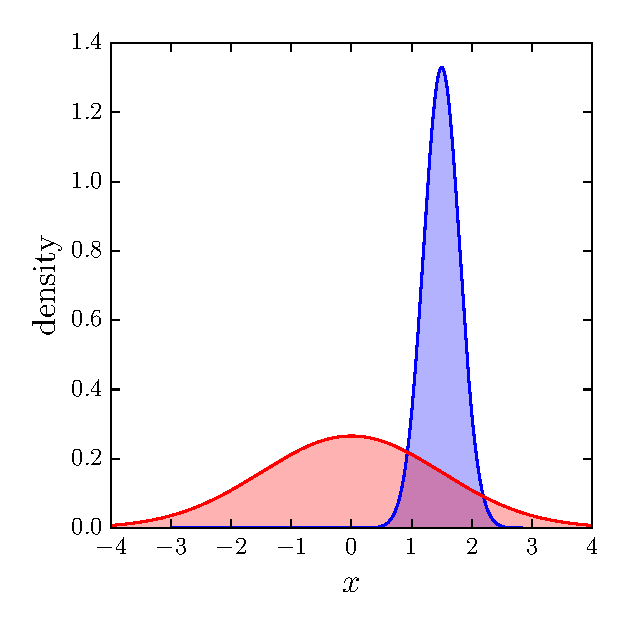
\includegraphics[width=0.23\textwidth]{hist_normal.pdf}
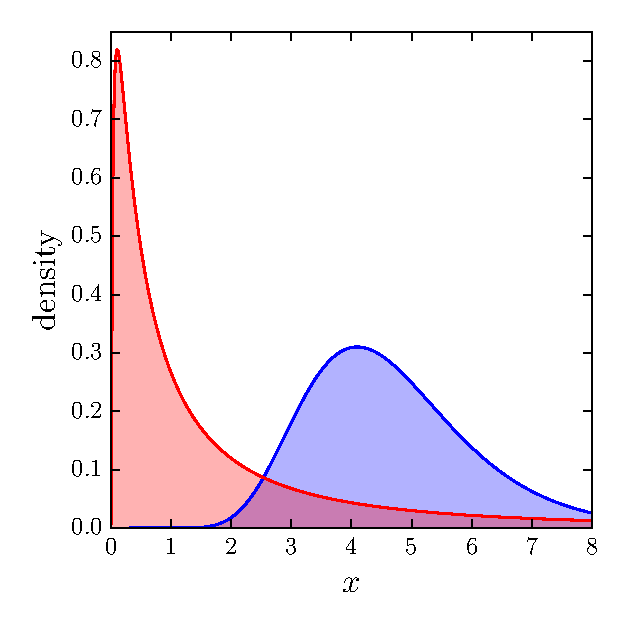
\includegraphics[width=0.23\textwidth]{hist_lognormal.pdf}\\[-0.6em]
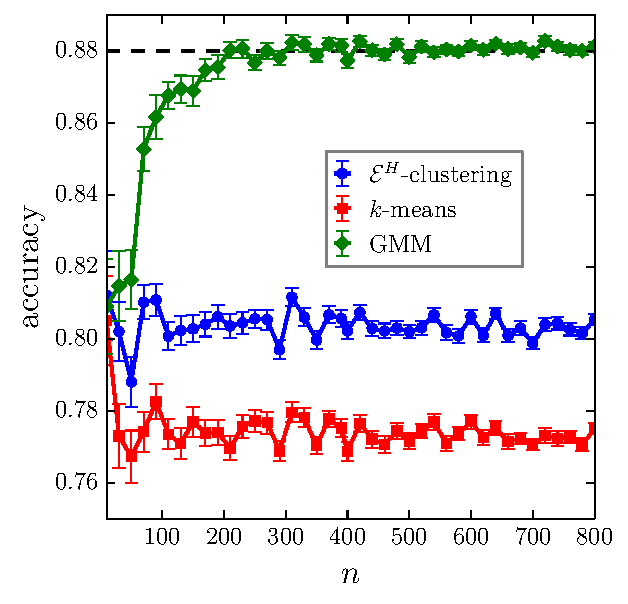
\includegraphics[width=0.23\textwidth]{1D_normal.pdf}
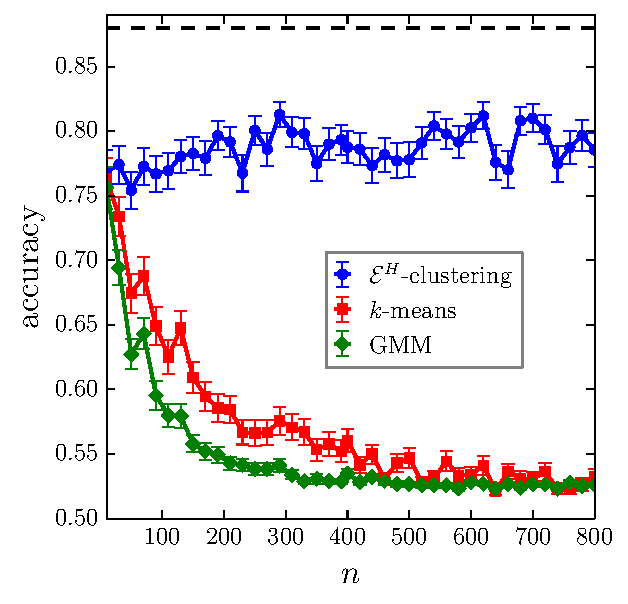
\includegraphics[width=0.23\textwidth]{1D_lognormal.pdf}
\caption{
\label{fig:1D}
Clustering results for one dimensional data
\eqref{eq:uni_normal}--\eqref{eq:uni_params}. \emph{Top Left:} Probability
density of \eqref{eq:uni_normal}. \emph{Top Right:} Probability
density of \eqref{eq:uni_lognormal}.
\emph{Bottom Left:} Clustering data from \eqref{eq:uni_normal}.
\emph{Bottom Right:} Clustering data from \eqref{eq:uni_lognormal}.
The dashed lines show the optimal Bayes accuracy, which in both cases 
are $\approx 0.88$.
}
\end{figure}

The first two experiments involve univariate
normal and lognormal mixtures:
\begin{align}
x &\stackrel{iid}{\sim} \tfrac{1}{2}
\mathcal{N}(\mu_1,\sigma_1^2) + 
\tfrac{1}{2} \mathcal{N}(\mu_2,\sigma_2^2) \label{eq:uni_normal} \\
x & \stackrel{iid}{\sim} \tfrac{1}{2}
\exp\left\{ \mathcal{N}(\mu_1,\sigma_1^2) \right\} + 
\tfrac{1}{2} \exp \left\{ \mathcal{N}(\mu_2,\sigma_2^2)\right\} 
\label{eq:uni_lognormal} \\
\mu_1 &= 1.5, \ \sigma_1=0.3, \ \mu_2=0, \ \sigma_2=1.5.
\label{eq:uni_params}
\end{align}
We increase the sample size $n$ and show clustering accuracy 
\eqref{eq:accuracy}
versus $n$ in Fig.~\ref{fig:1D}. $\mathcal{E}^H$-clustering 
performs better than $k$-means for normally distributed data, 
and worse than GMM,
as expected. 
However, for lognormal distributions $k$-means and GMM are only slightly
better than chance while $\mathcal{E}^H$-clustering is still 
accurate. The reason is that $k$-means and GMM models are inconsistent
with this lognormal data. Energy clustering on the other hand
is model-free.

\begin{figure}
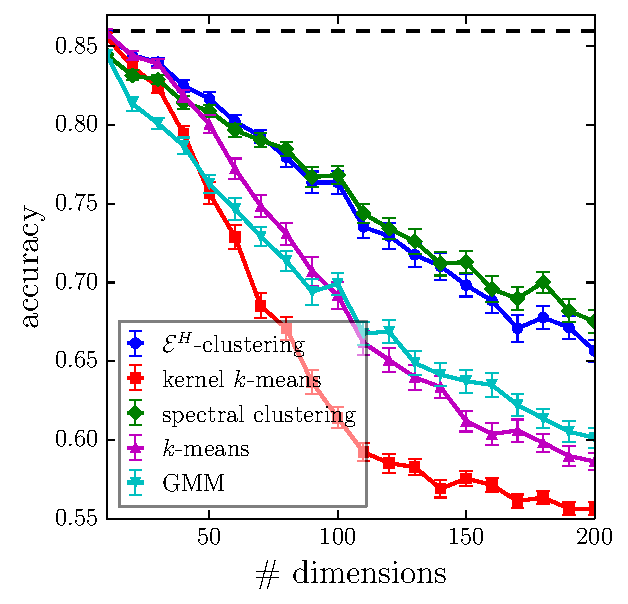
\includegraphics[width=0.23\textwidth]{normal_highdim_mean.pdf}
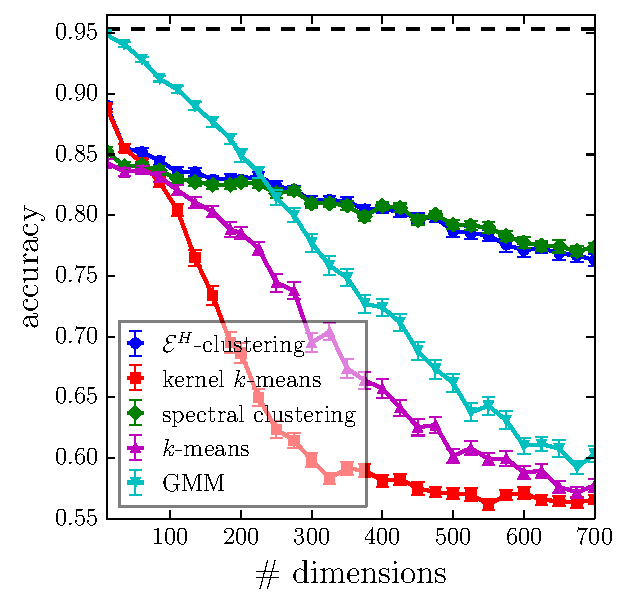
\includegraphics[width=0.23\textwidth]{normal_highdim_cov.pdf}
\caption{
\label{fig:gauss}
High dimensional Gaussian mixtures.
\emph{Left:} Parameters as in \eqref{eq:gauss1}.
\emph{Right:} Parameters  as in \eqref{eq:gauss2}. 
The dashed lines are Bayes accuracy.
}
\end{figure} 

Next we analyze
how the algorithms degrade as the number of dimensions increase.
Consider data from a Gaussian mixture
$x  \stackrel{iid}{\sim} 
\tfrac{1}{2} \mathcal{N}(\mu_1,\Sigma_1) +
\tfrac{1}{2} \mathcal{N}(\mu_2,\Sigma_2)$ in $\mathbb{R}^D$, with
$\Sigma_1=\Sigma_2 = I_D$,  and
\begin{equation}
\label{eq:gauss1}
\mu_1 = (\underbrace{0,\dotsc,0}_{\times D})^\top, \
\mu_2 = 0.7 (\underbrace{1,\dots,1}_{\times 10},
\underbrace{0,\dots,0}_{\times (D-10)})^\top.
\end{equation}
Bayes error is fixed as $D$ increases giving an optimal accuracy
of $\approx 0.86$.
We sample $200$ points on each trial.
As shown in Fig.~\ref{fig:gauss} (left), 
$\mathcal{E}^H$- and spectral clustering have close
performance,  
much better than kernel $k$-means, 
$k$-means and GMM. The improvement is noticeable in 
higher dimensions.
Still for a two-class Gaussian mixture we now choose
different numbers for the  diagonal covariance $\Sigma_2$.
We have $\Sigma_1=I_D$, $\mu_1=(0,\dotsc,0)^\top \in \mathbb{R}^D$,
$\mu_2=(1,\dotsc,1,0,\dotsc,0)^T \in \mathbb{R}^D$ 
with signal in the first $10$ dimensions, and
\begin{equation}
\label{eq:gauss2}
\begin{split}
\Sigma_2 &= \left( \begin{array}{c|c}
\widetilde{\Sigma}_{10} & 0 \\ \hline 
0 & I_{D-10} \end{array}\right), \\
\widetilde{\Sigma}_{10} &= \diag(1.367,  3.175,  3.247,  4.403,  1.249,\\
&\hspace{3.6em}1.969, 4.035,   4.237,  2.813,  3.637).
\end{split}
\end{equation}
We simply chose $10$ numbers uniformly at random between
$[1,5]$ and other choice would give analogous results.
Bayes  accuracy is fixed at $\approx 0.95$.
From Fig.~\ref{fig:gauss} (right) we see that 
GMM is better in low dimensions, 
but it quickly degenerates
as $D$ increases, as kernel $k$-means and $k$-means, while  
$\mathcal{E}^H$- and spectral clustering remains much more stable. 

\begin{figure}[t]
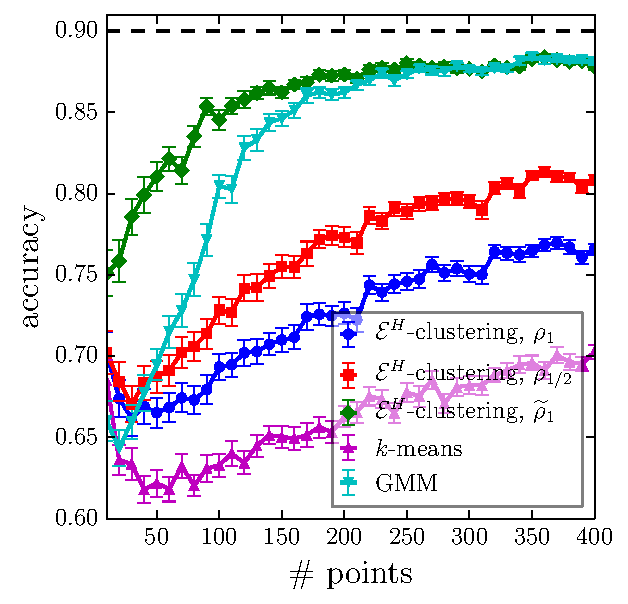
\includegraphics[width=0.23\textwidth]{normal_kernels.pdf}
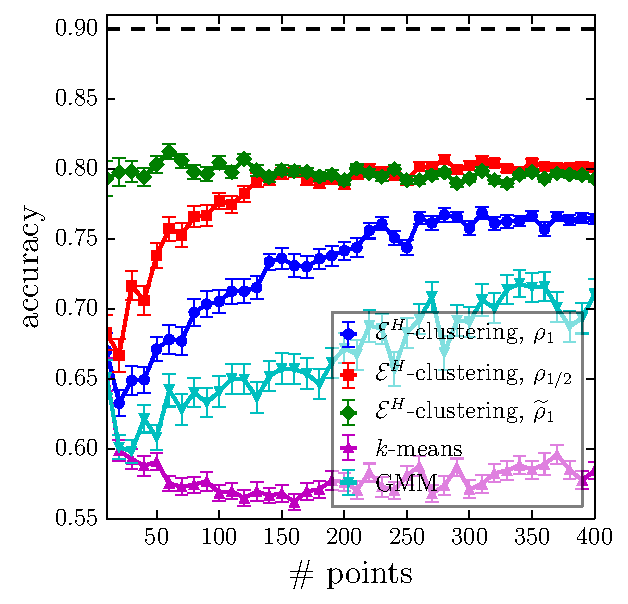
\includegraphics[width=0.23\textwidth]{lognormal_kernels.pdf}\\
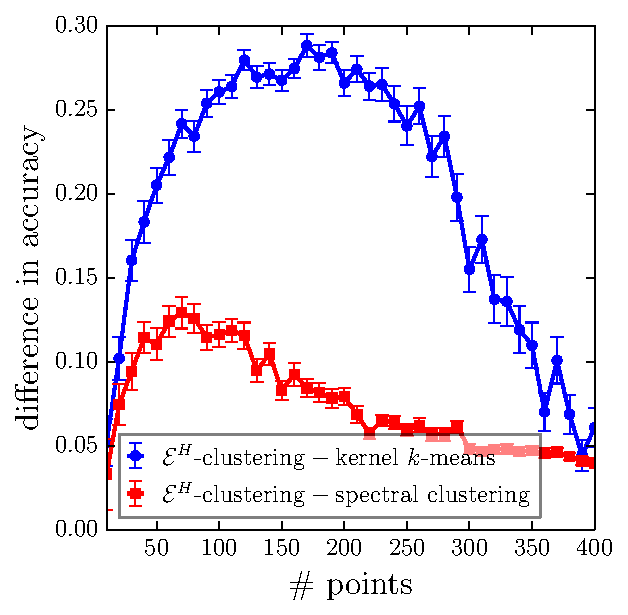
\includegraphics[width=0.23\textwidth]{normal_kernels_difference.pdf}
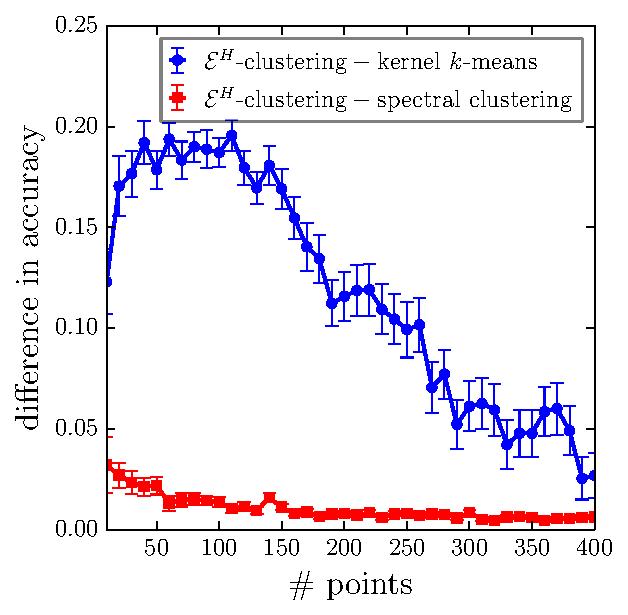
\includegraphics[width=0.23\textwidth]{lognormal_kernels_difference.pdf}
\caption{
\label{fig:consist}
Normal \emph{(Left)}
and lognormal \emph{(Right)} mixtures with
parameters \eqref{eq:20gauss}. We use different kernels
for $\mathcal{E}^H$-clustering. Bayes accuracy
is $\approx 0.9$.
The two plots in the \emph{Bottom} show the difference in accuracy
between $\mathcal{E}^H$-clustering versus kernel $k$-means and
spectral clustering, with $\widetilde{\rho}_1$.
}
\end{figure}


Consider
$x \stackrel{iid}{\sim} \tfrac{1}{2} \mathcal{N}(\mu_1,\Sigma_1)+
\tfrac{1}{2} \mathcal{N}(\mu_2, \Sigma_2)$ in $\mathbb{R}^{20}$ with 
$\Sigma_1=\tfrac{1}{2} I_{20}$, $\Sigma_2 = I_{20}$, and
\begin{equation}
\label{eq:20gauss}
\mu_1 = (\underbrace{0,\dotsc,0}_{\times 20})^\top ,\quad
\mu_2 = \tfrac{1}{2} 
(\underbrace{1,\dotsc,1}_{5},\underbrace{0,\dotsc,0}_{15})^\top.
\end{equation}
Bayes accuracy is $\approx 0.90$. 
We increase the sample size $n \in [10, 400]$ and show
the accuracy versus $n$ in Fig.~\ref{fig:consist} (top-left), where we compare
$\mathcal{E}^H$-clustering with different
kernels, indicated in the legend, to $k$-means and GMM.
Note that $\mathcal{E}^H$-clustering
with $\widetilde{\rho}_1$ is as accurate as GMM for large $n$ but
superior for small $n$. For
the same setting, in Fig.~\ref{fig:consist} (bottom-left) we
we show the difference in accuracy provided by $\mathcal{E}^H$-clustering minus
kernel $k$-means and spectral clustering when using $\widetilde{\rho}_1$.
$\mathcal{E}^H$-clustering was
always superior, otherwise there would be points with negative $y$-values.
Consider the same parameters as in \eqref{eq:20gauss} but now with
lognormal mixtures in $\mathbb{R}^D$.
The same experiments are shown in 
Fig.~\ref{fig:consist} (top-right and bottom-right), where
$\mathcal{E}^H$-clustering still performs accurately 
with any of those
kernels, contrary to $k$-means and GMM. 

\begin{figure}[b!]
\centering
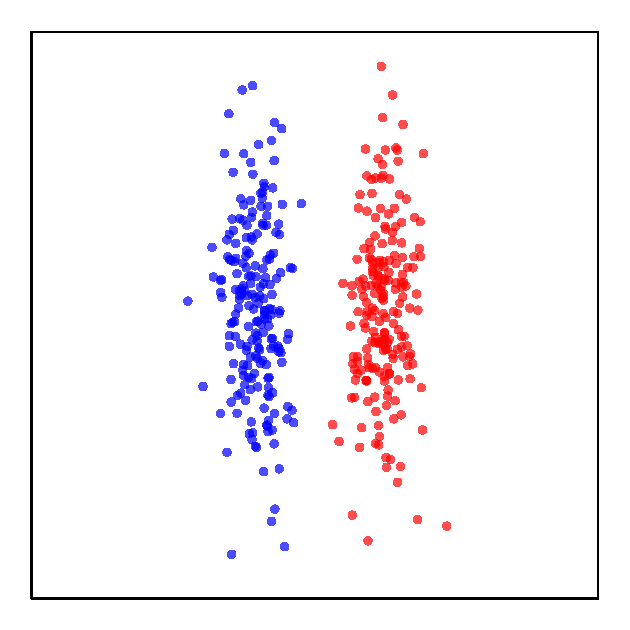
\includegraphics[width=0.15\textwidth]{2cigars.pdf}
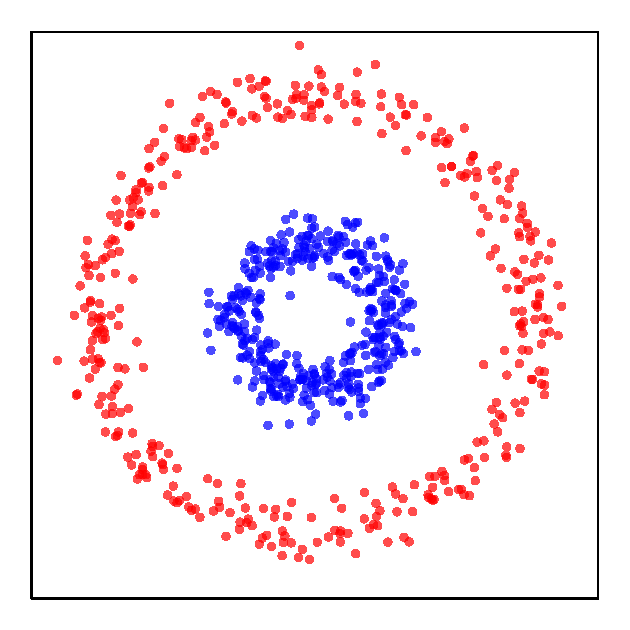
\includegraphics[width=0.15\textwidth]{2circles.pdf}
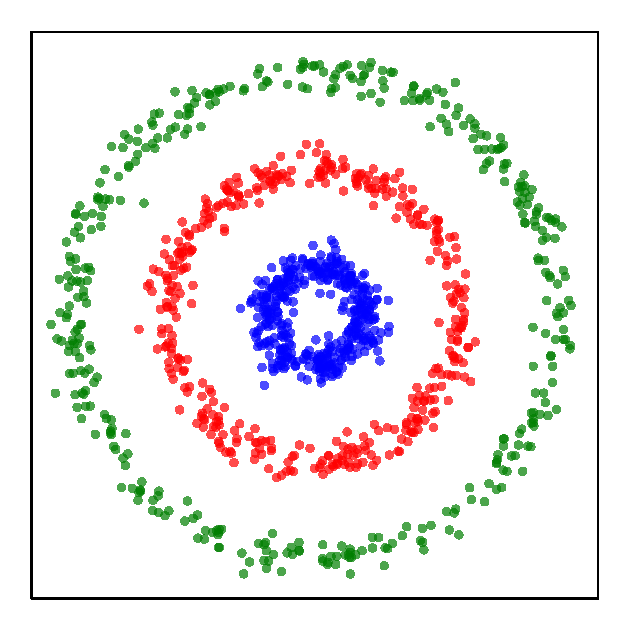
\includegraphics[width=0.15\textwidth]{3circles.pdf}
\caption{\label{fig:other}
\emph{Left}: Parallel cigars, $200$ points each. \emph{Center and Right:}
Two and three concentric circles, respectively,
with Gaussian noise. $400$ points for each class.
}
\end{figure}

\begin{table*}
\caption{\label{table:other}
Clustering data from Figure~\ref{fig:other}.
}
\begin{center}
\footnotesize{
\begin{tabular}{@{}r  l l  l l  l l@{}}
\toprule[1pt]
 & & \emph{Parallel Cigars}
 & & \emph{Two Circles}
 & & \emph{Three Circles} \\
\midrule[0.5pt]
\multirow{4}{*}{\emph{$\mathcal{E}^H$-clustering~~~~}}
& $\rho_{1}$ & $0.705\pm 0.065$
& $\rho_{1}$ & $0.521\pm 0.005$
& $\rho_{1}$ & $0.393\pm 0.020$ \\
& $\rho_{1/2}$ & $0.952\pm 0.048$
& $\rho_{1/2}$ & $0.522\pm 0.004$
& $\rho_{1/2}$ & $0.486\pm 0.040$ \\
& $\widetilde{\rho}_{2}$ & $\bm{0.9987\pm 0.0008}$
& $\widetilde{\rho}_{1}$ & $0.778\pm 0.075$
& $\widetilde{\rho}_{2}$ & $0.666\pm 0.007$ \\
& $\widehat{\rho}_{2}$  & $0.956\pm 0.020$
& $\widehat{\rho}_{1}$  & $\bm{1.0\pm 0.0}$
& $\widehat{\rho}_{2}$ & $\bm{0.676\pm 0.002}$ \\
\midrule[0.5pt]
\emph{spectral-clustering~~~~}
& $\widetilde{\rho}_{2}$ & $0.557\pm 0.014$ 
& $\widehat{\rho}_{1}$ & $0.732\pm 0.002$ 
& $\widehat{\rho}_{2}$ & $0.364\pm 0.004$  \\
\emph{$k$-means}~~~~ 
& \xmark & $0.550\pm 0.011$
& \xmark & $0.522\pm 0.004$
& \xmark & $0.368\pm 0.005$ \\
\emph{GMM}~~~~
& \xmark & $0.903\pm 0.064$
& \xmark & $0.595\pm 0.011$
& \xmark & $0.465\pm 0.030$ \\
\bottomrule[1pt]
\end{tabular}
}
\end{center}
\end{table*}

In Fig.~\ref{fig:other} we have examples of
complex two dimensional datasets. 
We apply $\mathcal{E}^H$-clustering  with different kernel choices,
and also spectral clustering with the best kernel choice, besides 
$k$-means and GMM. Here we perform only $10$ Monte Carlo runs.
For parallel cigars we initialize
all algorithms with $k$-means++, and the concentric circles example
we initialize at random.
The results are shown in Table~\ref{table:other}.
$\mathcal{E}^H$-clustering has superior performance
in every example, in particular better than the
spectral clustering.
For parallel cigars the metrics $\rho_1$ and $\rho_{1/2}$ still provide
accurate results, however, for
the concentric circles the kernel choice is more sensitive.

\subsection{Real Data Experiment}


\begin{figure*}
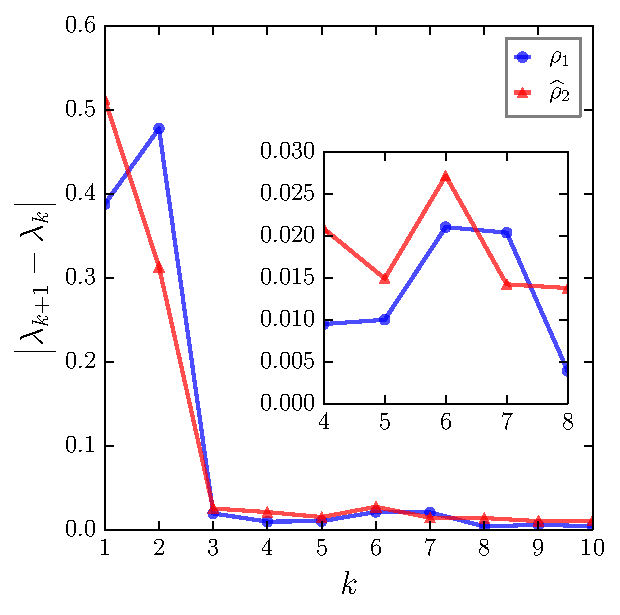
\includegraphics[width=0.18\textwidth]{eigen_gap.pdf}
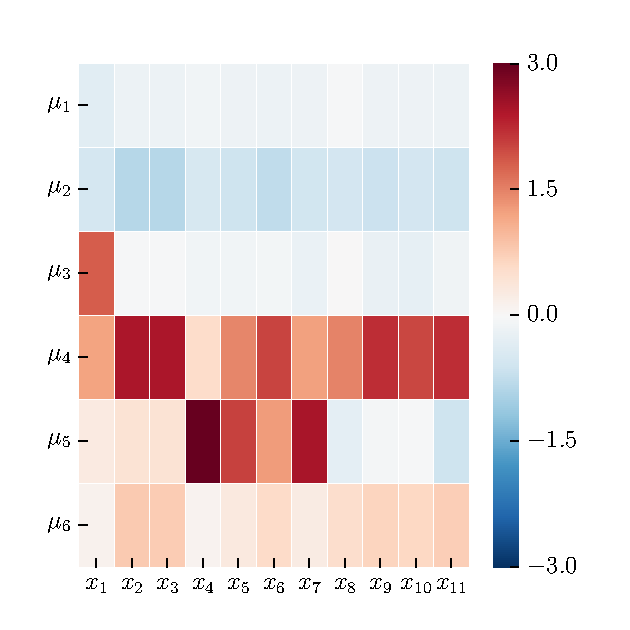
\includegraphics[width=0.2\textwidth]{heat_means_k6_energy.pdf}
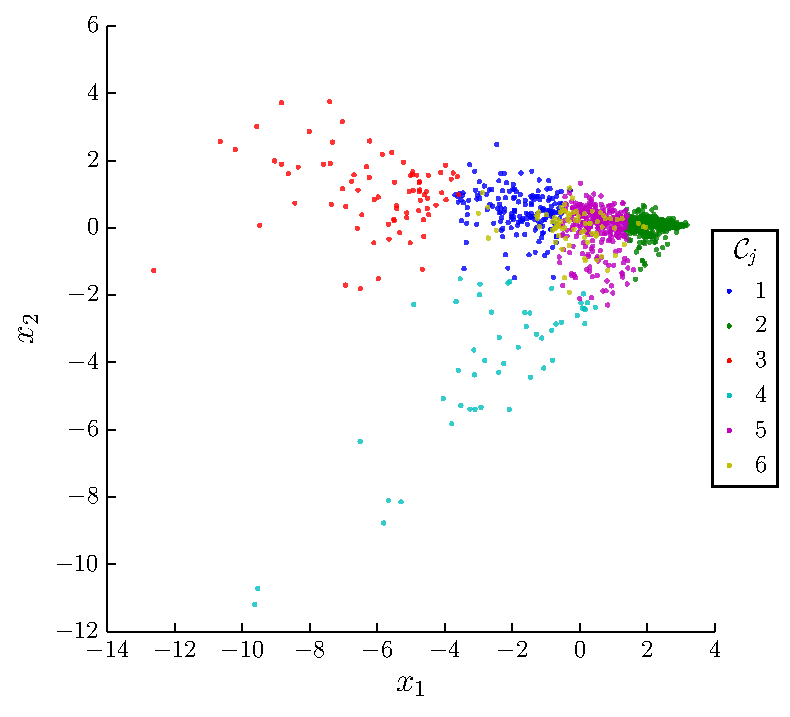
\includegraphics[width=0.2\textwidth]{synapse_cluster_2d_k6_energy.pdf}
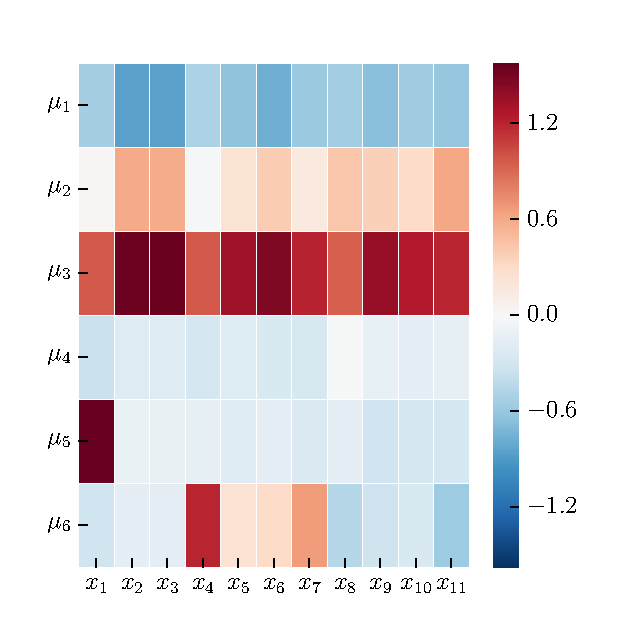
\includegraphics[width=0.2\textwidth]{heat_means_k6_gauss.pdf}
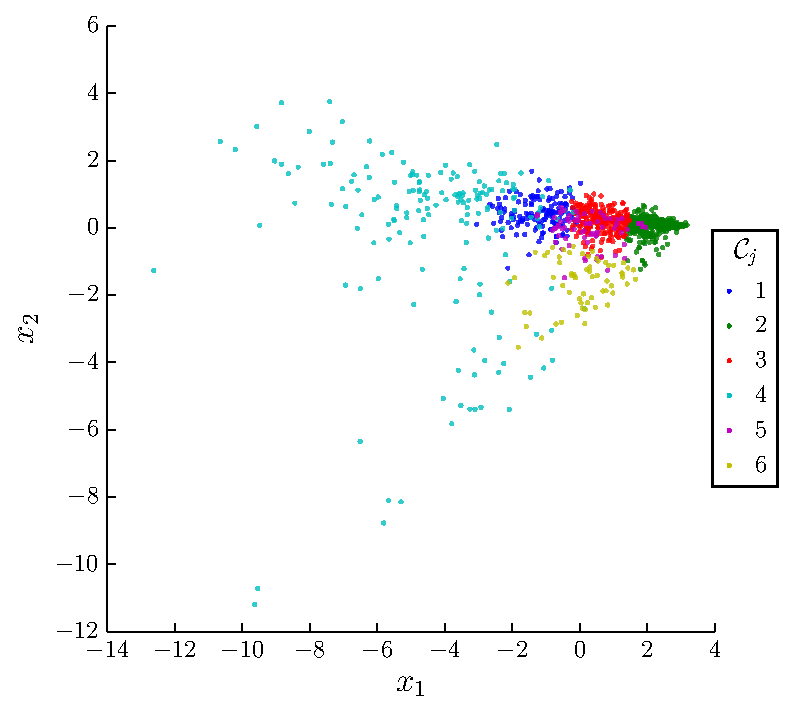
\includegraphics[width=0.2\textwidth]{synapse_cluster_2d_k6_gauss.pdf}
\vspace{-0.8cm}
\caption{\label{fig:synapse}
Clustering synapse dataset.
Plots in order from \emph{left} to \emph{right}.
\emph{First:} Eigenvalues of random walk Laplacian. We choose
$k=6$ since its the first time we see a peak. We use energy clustering
with the two metrics $\rho_1$ and $\widehat{\rho}_2$; see
\eqref{eq:test_metrics}.
\emph{Second:} Heat map of the cluster means versus features
using energy clustering with standard
metric $\rho_1$ from energy statistics.
\emph{Third:} Clustered points projected into the two principal components,
using $\rho_1$.
\emph{Fourth:} Heat map of the cluster means versus features
using energy clustering with Gaussian metric 
$\widehat{\rho}_2$.
\emph{Fifth:} Clustered points projected into the two principal components,
using $\widehat{\rho}_2$.
}
\end{figure*}


The considered dataset 
describes protein expression of neural synapses (chemical 
connections between neurons), being
crucial for understanding the diversity of synapses. This is
part of a large NIH funded consortium within the BRAIN initiative;
we refer to \citet{Collman2015} for details.
We have $1025$ data points
with $11$ features. Each point
corresponds to a $(x,y,z)$ location in the brain. We normalize this
dataset before applying $\mathcal{E}^H$-clustering.

We use the two
metrics $\rho_1$ and $\widehat{\rho}_2$; see \eqref{eq:test_metrics}.
We compute the difference between eigenvalues of the random walk Laplacian
obtained from the kernel matrix $G$ \eqref{eq:kernel_matrix}.
The choice of $k$ corresponds to the first time we see a meaningful
peak in the plot, which occurs at $k=6$; first plot in
Fig.~\ref{fig:synapse}.
This procedure to find $k$ is common in the literature \cite{vonLuxburg2007}.
Having found $k$ we now cluster the data.
First we use the metric $\rho_1$, which
is the standard Euclidean choice in energy statistics.
In the second and third plots of Fig.~\ref{fig:synapse} we show a heat
map of the cluster means versus features and the clustered data points
projected into the 2 principal components, respectively.
The fourth and fifth plots in Fig.~\ref{fig:synapse} show the same
experiment but using the metric $\widehat{\rho}_2$ corresponding
to a Gaussian kernel.

We remark that we also used the gap statistic \cite{Tibshirani2001} based
on $k$-means to determine the number of clusters as a comparison.
The results slightly suggest $k=6$, but it does not pass the gap
statistic test. 



%%%%%%%%%%%%%%%%%%%%%%%%%%%%%%%%%%%%%%%%%%%%%%%%%%%%%%%%%%%%%%%%%%%%%%%%%%%%%%%
\section{Final Remarks}
\label{sec:conclusion}

We proposed clustering from the perspective of generalized energy
statistics, valid for arbitrary spaces of negative type.
Our mathematical formulation yields
a QCQP in the associated RKHS;
Proposition~\ref{th:qcqp2}.
We showed that such QCQP
is equivalent to kernel $k$-means optimization problem, 
once the kernel is fixed; 
Proposition~\ref{th:kernel_kmeans}. However, energy statistics fixes
a family of standard kernels in Euclidean space, and
more general kernels 
on spaces of negative type as well.

We proposed the iterative $\mathcal{E}^H$-clustering 
(Algorithm~\ref{algo})
which is 
a kernelized version of Hartigan's method. 
It was compared to kernel $k$-means algorithm,
based on Lloyd's heuristic.
Both have the same complexity, however, numerical and theoretical
results provide compelling evidence that $\mathcal{E}^H$-clustering
is more robust with superior performance, specially in high
dimensions. 
Moreover, $\mathcal{E}^H$-clustering with standard kernels from energy
statistics outperformed $k$-means and GMM
on several settings, even on Gaussian ones.
In some cases
$\mathcal{E}^H$-clustering also surpassed spectral clustering, and in
others performed similarly but never worse. 
Note that computing eigenvectors
of large matrices can be unfeasible and iterative methods are preferred.
We provided an application of $\mathcal{E}^H$-clustering to an
important real dataset
describing protein expression of neural synapses.
Finally, we remark that kernel methods can benefit from sparsity and
fixed-rank approximations of the Gram matrix and there is plenty
of room to make $\mathcal{E}^H$-clustering more scalable.


%\subsection*{Acknowledgements}
%We would like to thank Carey Priebe 
%for discussions.
%We would like to acknowledge the support of the Transformative
%Research Award (NIH \#R01NS092474) and  the Defense Advanced Research Projects
%Agency’s (DARPA) SIMPLEX program through SPAWAR contract N66001-15-C-4041.


\bibliographystyle{icml2018}
\bibliography{biblio.bib}

\clearpage

\appendix

\section{Supplementary Material}

Here we collect the proofs of our main results.

\begin{proof}[Proof of Lemma~\ref{th:minimize}]
From \eqref{eq:within} and \eqref{eq:between}
we have
\begin{equation}
\begin{split}
S + W &= 
\dfrac{1}{2n} \sum_{\substack{i,j=1 \\ i\ne j}}^k n_i n_j g(\C_i, \C_j)
\\&+ \dfrac{1}{2n} \sum_{i=1}^{k} 
\bigg[ n - 
\sum_{j\ne i = 1}^k n_j \bigg] 
n_i g(\C_i, \C_i) \\
& = \dfrac{1}{2n} \sum_{i,j=1}^k n_i n_j g(\C_i, \C_j) \\
&= \dfrac{1}{2n} \sum_{x \in \mathbb{X}} \sum_{y \in \mathbb{X}} \rho(x,y)\\
&= \dfrac{n}{2} g(\mathbb{X}, \mathbb{X}).
\end{split}
\end{equation}
Note that the right hand side of this equation 
only depends on the pooled data, so it is a constant
independent of the choice of partition. Therefore, maximizing
$S$ over the choice of partition is equivalent to minimizing $W$.
\end{proof}

\begin{proof}[Proof of Proposition~\ref{th:qcqp2}]
From 
\eqref{eq:gen_kernel},
\eqref{eq:g_def}, and
\eqref{eq:within}
we have
\begin{equation}
\label{eq:W2}
\begin{split}
W
&= \dfrac{1}{2} \sum_{j=1}^k \dfrac{1}{n_j} \sum_{x,y \in \C_j} \rho(x,y) \\
&= \sum_{j=1}^k \sum_{x \in \C_j}  \bigg(
\kk(x,x) - \dfrac{1}{n_j} \sum_{y \in \C_j} \kk(x,y) \bigg).
\end{split}
\end{equation}
Note that the first term is global so it does not contribute to the 
optimization problem.
Therefore, minimizing \eqref{eq:W2} is equivalent to
\begin{equation}
\label{eq:max_prob}
\max_{ \C_1,\dotsc,\C_k } 
\sum_{j=1}^k \dfrac{1}{n_j} \sum_{x,y\in C_j} \kk(x,y) .
\end{equation}
But 
\begin{equation}
\sum_{x, y \in \C_j} \kk(x, y) =
\sum_{p=1}^{n} \sum_{q=1}^{n} Z_{pj} Z_{qj} G_{pq} = 
(Z^\top G \, Z)_{jj},
\end{equation}
where we used the definitions \eqref{eq:kernel_matrix} and
\eqref{eq:label_matrix}. 
Notice that $n_j^{-1} = D^{-1}_{jj}$, where the diagonal matrix $D = 
\diag(n_1,\dotsc,n_k)$ contains the number of points in each cluster, 
thus the objective function in 
\eqref{eq:max_prob} is equal to $\sum_{j=1}^k D^{-1}_{jj} 
\left( Z^\top G Z \right)_{jj} = \Tr \left( D^{-1} Z^\top G Z \right)$. 
Now we can
use the cyclic property
of the trace, and by the  definition of the matrix $Z$
in \eqref{eq:label_matrix}, we obtain the following integer
programing problem:
\begin{equation}\label{eq:qcqp}
\begin{split}
&\max_{Z} \Tr\Big( \big( Z D^{-1/2}\big)^\top G 
\big( ZD^{-1/2} \big) 
\Big) \\
&\mbox{s.t. $Z_{ij} \in \{0,1\}$, $\sum_{j=1}^k Z_{ij} = 1$, 
$\sum_{i=1}^n Z_{ij} = n_j$.}
\end{split}
\end{equation}

Now we write this in terms of the matrix $Y = Z D^{-1/2}$.
The objective function immediately becomes
$\Tr\left( Y^\top G \, Y\right)$. Notice that the above constraints
imply that $Z^T Z = D$, which in turn gives
$D^{-1/2} Y^T Y D^{-1/2} = D$, or $Y^\top Y = I$. 
Also, every entry of $Y$ is positive by definition,
$Y \ge 0$. Now it only remains to show the last 
constraint in \eqref{eq:qcqp2}, which comes from the last
constraint in \eqref{eq:qcqp}. In matrix form this reads
$Z^T \e = D \e$. Replacing $Z=YD^{1/2}$ we have
$Y^\top \e = D^{1/2} \e$. Multiplying this last equation
on the left by $Y$, and noticing
that $Y D^{1/2} \e = Z \e = \e$, we finally obtain
$Y Y^\top \e = \e$. Therefore, the optimization 
problem \eqref{eq:qcqp} is equivalent
to \eqref{eq:qcqp2} .
\end{proof}

\begin{proof}[Proof of Proposition~\ref{th:kernel_kmeans}]
Notice that 
\begin{equation}
\begin{split}
\| \varphi(x) - \varphi(\mu_j) \|^2 &= \langle 
\varphi(x),  \varphi(x) \rangle
- 2 \langle \varphi(x), \varphi(\mu_j)\rangle \\
& \qquad + \langle \varphi(\mu_j), \varphi(\mu_j) \rangle,
\end{split}
\end{equation}
therefore, kernel $k$-means objective function becomes
\begin{equation}
\label{eq:J}
\begin{split}
\sum_{j=1}^k \sum_{x\in\C_j} \bigg(
\kk(x,x) - 
\dfrac{2}{n_j} \sum_{y\in \C_j} \kk(x,y) \\
+ \dfrac{1}{n_j^2}
\sum_{y,z \in \C_j} \kk(y,z) \bigg).
\end{split}
\end{equation}
The first term is global so it does not contribute to the optimization
problem. Notice that the third term gives
$\sum_{x\in\C_j} \tfrac{1}{n_j^2} \sum_{y,z\in\C_j} \kk(y,z) =
\tfrac{1}{n_j}\sum_{y,z\in\C_j} \kk(y,z)$, which is the same as
the second term. Thus, problem
\eqref{eq:kernel_kmeans} is equivalent to
\begin{equation}
\max_{\C_1,\dotsc,\C_k}
\sum_{j=1}^k \dfrac{1}{n_j} \sum_{x,y \in\C_j} \kk(x,y) 
\end{equation}
which is exactly the same as 
\eqref{eq:max_prob} from the energy statistics formulation. Therefore,
once the kernel $\kk$ is fixed, the function 
$W$ given by \eqref{eq:within} is the same
as $J$ in \eqref{eq:kernel_kmeans}.
The remaining of the proof proceeds as 
already shown in the proof of Proposition~\ref{th:qcqp2}, leading to
the optimization problem \eqref{eq:qcqp2}.
\end{proof}

\end{document}

